\documentclass[tikz,border=8pt]{standalone}
\usepackage{amsmath}
\usetikzlibrary{arrows.meta}
\definecolor{ink}{HTML}{21352F}
\definecolor{teal}{HTML}{087F7B}
\definecolor{blue}{HTML}{4B77A8}
\definecolor{gold}{HTML}{C58B2A}
\definecolor{rose}{HTML}{B65A62}
\begin{document}
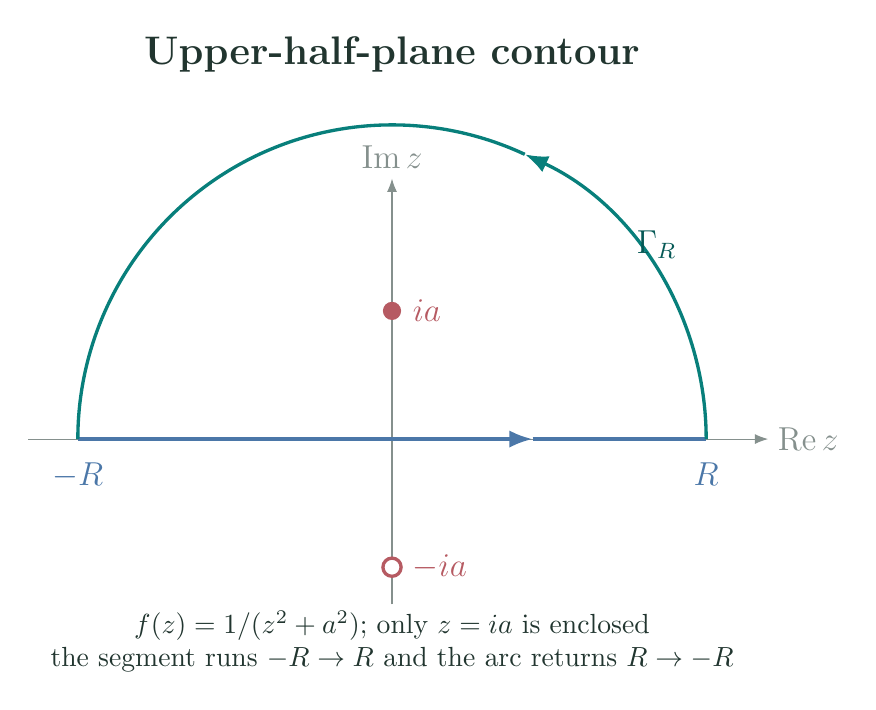
\begin{tikzpicture}[font=\large\sffamily,text=ink,>=Latex,scale=1.05]
  \node[font=\bfseries\Large] at (0,4.65)
    {Upper-half-plane contour};
  \draw[->,ink!55] (-4.4,0)--(4.55,0) node[right] {$\operatorname{Re}z$};
  \draw[->,ink!55] (0,-2.0)--(0,3.15) node[above] {$\operatorname{Im}z$};
  \draw[blue,very thick,->] (-3.8,0)--(1.7,0);
  \draw[blue,very thick] (1.7,0)--(3.8,0);
  \draw[teal,very thick,->] (3.8,0)
    arc[start angle=0,end angle=65,radius=3.8];
  \draw[teal,very thick] ({3.8*cos(65)},{3.8*sin(65)})
    arc[start angle=65,end angle=180,radius=3.8];
  \fill[rose] (0,1.55) circle (.11);
  \node[rose,right=4pt] at (0,1.55) {$ia$};
  \fill[white,draw=rose,very thick] (0,-1.55) circle (.11);
  \node[rose,right=4pt] at (0,-1.55) {$-ia$};
  \node[blue,below=5pt] at (-3.8,0) {$-R$};
  \node[blue,below=5pt] at (3.8,0) {$R$};
  \node[teal!70!black] at (3.2,2.35) {$\Gamma_R$};
  \node[font=\normalsize,align=center] at (0,-2.45)
    {$f(z)=1/(z^2+a^2)$; only $z=ia$ is enclosed\\
     the segment runs $-R\to R$ and the arc returns $R\to-R$};
\end{tikzpicture}
\end{document}
